\documentclass[]{article}
\usepackage{lmodern}
\usepackage{amssymb,amsmath}
\usepackage{ifxetex,ifluatex}
\usepackage{fixltx2e} % provides \textsubscript
\ifnum 0\ifxetex 1\fi\ifluatex 1\fi=0 % if pdftex
  \usepackage[T1]{fontenc}
  \usepackage[utf8]{inputenc}
\else % if luatex or xelatex
  \ifxetex
    \usepackage{mathspec}
  \else
    \usepackage{fontspec}
  \fi
  \defaultfontfeatures{Ligatures=TeX,Scale=MatchLowercase}
\fi
% use upquote if available, for straight quotes in verbatim environments
\IfFileExists{upquote.sty}{\usepackage{upquote}}{}
% use microtype if available
\IfFileExists{microtype.sty}{%
\usepackage{microtype}
\UseMicrotypeSet[protrusion]{basicmath} % disable protrusion for tt fonts
}{}
\usepackage[margin=1in]{geometry}
\usepackage{hyperref}
\hypersetup{unicode=true,
            pdftitle={Report Template coursework assignment A - 2018},
            pdfauthor={Þórunn Arna Ómardóttir (4917499), Nathan Buskulic (4947916), Mitchell Deen(4396340)},
            pdfborder={0 0 0},
            breaklinks=true}
\urlstyle{same}  % don't use monospace font for urls
\usepackage{color}
\usepackage{fancyvrb}
\newcommand{\VerbBar}{|}
\newcommand{\VERB}{\Verb[commandchars=\\\{\}]}
\DefineVerbatimEnvironment{Highlighting}{Verbatim}{commandchars=\\\{\}}
% Add ',fontsize=\small' for more characters per line
\usepackage{framed}
\definecolor{shadecolor}{RGB}{248,248,248}
\newenvironment{Shaded}{\begin{snugshade}}{\end{snugshade}}
\newcommand{\KeywordTok}[1]{\textcolor[rgb]{0.13,0.29,0.53}{\textbf{#1}}}
\newcommand{\DataTypeTok}[1]{\textcolor[rgb]{0.13,0.29,0.53}{#1}}
\newcommand{\DecValTok}[1]{\textcolor[rgb]{0.00,0.00,0.81}{#1}}
\newcommand{\BaseNTok}[1]{\textcolor[rgb]{0.00,0.00,0.81}{#1}}
\newcommand{\FloatTok}[1]{\textcolor[rgb]{0.00,0.00,0.81}{#1}}
\newcommand{\ConstantTok}[1]{\textcolor[rgb]{0.00,0.00,0.00}{#1}}
\newcommand{\CharTok}[1]{\textcolor[rgb]{0.31,0.60,0.02}{#1}}
\newcommand{\SpecialCharTok}[1]{\textcolor[rgb]{0.00,0.00,0.00}{#1}}
\newcommand{\StringTok}[1]{\textcolor[rgb]{0.31,0.60,0.02}{#1}}
\newcommand{\VerbatimStringTok}[1]{\textcolor[rgb]{0.31,0.60,0.02}{#1}}
\newcommand{\SpecialStringTok}[1]{\textcolor[rgb]{0.31,0.60,0.02}{#1}}
\newcommand{\ImportTok}[1]{#1}
\newcommand{\CommentTok}[1]{\textcolor[rgb]{0.56,0.35,0.01}{\textit{#1}}}
\newcommand{\DocumentationTok}[1]{\textcolor[rgb]{0.56,0.35,0.01}{\textbf{\textit{#1}}}}
\newcommand{\AnnotationTok}[1]{\textcolor[rgb]{0.56,0.35,0.01}{\textbf{\textit{#1}}}}
\newcommand{\CommentVarTok}[1]{\textcolor[rgb]{0.56,0.35,0.01}{\textbf{\textit{#1}}}}
\newcommand{\OtherTok}[1]{\textcolor[rgb]{0.56,0.35,0.01}{#1}}
\newcommand{\FunctionTok}[1]{\textcolor[rgb]{0.00,0.00,0.00}{#1}}
\newcommand{\VariableTok}[1]{\textcolor[rgb]{0.00,0.00,0.00}{#1}}
\newcommand{\ControlFlowTok}[1]{\textcolor[rgb]{0.13,0.29,0.53}{\textbf{#1}}}
\newcommand{\OperatorTok}[1]{\textcolor[rgb]{0.81,0.36,0.00}{\textbf{#1}}}
\newcommand{\BuiltInTok}[1]{#1}
\newcommand{\ExtensionTok}[1]{#1}
\newcommand{\PreprocessorTok}[1]{\textcolor[rgb]{0.56,0.35,0.01}{\textit{#1}}}
\newcommand{\AttributeTok}[1]{\textcolor[rgb]{0.77,0.63,0.00}{#1}}
\newcommand{\RegionMarkerTok}[1]{#1}
\newcommand{\InformationTok}[1]{\textcolor[rgb]{0.56,0.35,0.01}{\textbf{\textit{#1}}}}
\newcommand{\WarningTok}[1]{\textcolor[rgb]{0.56,0.35,0.01}{\textbf{\textit{#1}}}}
\newcommand{\AlertTok}[1]{\textcolor[rgb]{0.94,0.16,0.16}{#1}}
\newcommand{\ErrorTok}[1]{\textcolor[rgb]{0.64,0.00,0.00}{\textbf{#1}}}
\newcommand{\NormalTok}[1]{#1}
\usepackage{longtable,booktabs}
\usepackage{graphicx,grffile}
\makeatletter
\def\maxwidth{\ifdim\Gin@nat@width>\linewidth\linewidth\else\Gin@nat@width\fi}
\def\maxheight{\ifdim\Gin@nat@height>\textheight\textheight\else\Gin@nat@height\fi}
\makeatother
% Scale images if necessary, so that they will not overflow the page
% margins by default, and it is still possible to overwrite the defaults
% using explicit options in \includegraphics[width, height, ...]{}
\setkeys{Gin}{width=\maxwidth,height=\maxheight,keepaspectratio}
\IfFileExists{parskip.sty}{%
\usepackage{parskip}
}{% else
\setlength{\parindent}{0pt}
\setlength{\parskip}{6pt plus 2pt minus 1pt}
}
\setlength{\emergencystretch}{3em}  % prevent overfull lines
\providecommand{\tightlist}{%
  \setlength{\itemsep}{0pt}\setlength{\parskip}{0pt}}
\setcounter{secnumdepth}{5}
% Redefines (sub)paragraphs to behave more like sections
\ifx\paragraph\undefined\else
\let\oldparagraph\paragraph
\renewcommand{\paragraph}[1]{\oldparagraph{#1}\mbox{}}
\fi
\ifx\subparagraph\undefined\else
\let\oldsubparagraph\subparagraph
\renewcommand{\subparagraph}[1]{\oldsubparagraph{#1}\mbox{}}
\fi

%%% Use protect on footnotes to avoid problems with footnotes in titles
\let\rmarkdownfootnote\footnote%
\def\footnote{\protect\rmarkdownfootnote}

%%% Change title format to be more compact
\usepackage{titling}

% Create subtitle command for use in maketitle
\newcommand{\subtitle}[1]{
  \posttitle{
    \begin{center}\large#1\end{center}
    }
}

\setlength{\droptitle}{-2em}

  \title{Report Template coursework assignment A - 2018}
    \pretitle{\vspace{\droptitle}\centering\huge}
  \posttitle{\par}
  \subtitle{CS4125 Seminar Research Methodology for Data Science}
  \author{Þórunn Arna Ómardóttir (4917499), Nathan Buskulic (4947916), Mitchell
Deen(4396340)}
    \preauthor{\centering\large\emph}
  \postauthor{\par}
      \predate{\centering\large\emph}
  \postdate{\par}
    \date{4/3/2019}


\begin{document}
\maketitle

\tableofcontents

\section{Part 1 - Design and set-up of true
experiment}\label{part-1---design-and-set-up-of-true-experiment}

\subsection{The motivation for the planned
research.}\label{the-motivation-for-the-planned-research.}

(Max 250 words) The coffee is today the most consumed drink in the world
and it is told to increase your performance and concentration. We want
to challenge this idea and verify scientifically if this is a valid
idea. We want to test how coffee consumption (and the level of caffeine
inside) affect the result of an IQ test. We are most interesting and
seeing what the affect is on TU Delft students like ourselves. So the
participants will be recruited from the TU Delft student body. \# Add
that we are doing that on tudelft student

\subsection{The theory underlying the
research.}\label{the-theory-underlying-the-research.}

(Max 250 words) Preferable based on theories reported in literature
There is a large body of literature available on the effects of caffeine
on the performance in cognitive tasks. Literature generally supports the
idea that coffee improves this performance, see e.g. (Jarvis, 1993;
Nehlig, 2010; Rogers et al., 2008). In a brief survey of the relevant
literature we did not find any studies specifically addressing students.
We would like to investigate this part of the population in more detail.

Jarvis, M. J. (1993). Does caffeine intake enhance absolute levels of
cognitive performance?. Psychopharmacology, 110(1-2), 45-52. Rogers, P.
J., Smith, J. E., Heatherley, S. V., \& Pleydell-Pearce, C. W. (2008).
Time for tea: mood, blood pressure and cognitive performance effects of
caffeine and theanine administered alone and together.
Psychopharmacology, 195(4), 569. Nehlig, A. (2010). Is caffeine a
cognitive enhancer?. Journal of Alzheimer's Disease, 20(s1), S85-S94.

\subsection{Research questions}\label{research-questions}

The research question that will be examined in the experiment (or
alternatively the hypothesis that will be tested in the experiment) Does
coffee consumption increases IQ test score \#Should we add the caffeine
level ?

\subsection{The related conceptual
model}\label{the-related-conceptual-model}

This model should include: \emph{Independent variable(s) -\textgreater{}
Coffee consumption }Dependent variable -\textgreater{} score at IQ test.
\emph{Mediating variable (at least 1) -\textgreater{} sleepingness
feeling }Moderating variable (at least 1) -\textgreater{} amount of
caffeine, prior coffee consumption habit/caffeine tolerance

\subsection{Experimental Design}\label{experimental-design}

Note that the study should have a true experimental design The
experiment is a two groups, post test only, randomized controlled trail.

\subsection{Experimental procedure}\label{experimental-procedure}

Describe how the experiment will be executed step by step The
participants will be separated into two groups randomly. One group will
do the IQ test without any prior coffee consumption while the second
group will do the test half an hour after coffee consumption. In the
coffe consumption groups, participants will be separated in three
subgroups where they will get coffe with different caffeine level. This
will allow us to measure the general impact of drinking coffee on an IQ
test but it will also allow us to test the difference between each
caffeine level.

\subsection{Measures}\label{measures}

Describe the measure that will be used The Coffe consumption will be
measured in ml. The perfomance in an IQ test will in a simple integer
number on the scale from 0-200 where the mean is around 100.
Sleepingness will be given by the participants on the scale from 0-10
where 10 means the highest level of sleepingness. The amount of caffeine
will be measured in mg. Prior coffeedrinking habits will be given by
participants. They will be asked how much coffee they typically drink on
a normal day.

\subsection{Participants}\label{participants}

Describe which participants will recruit in the study and how they will
be recruited

Since we are just going to make this experiment on the effects of coffee
consumption on students at TU Delft we need to find participants from
that group of people. Emails will be sent out to the student body
explaining the theory of the experiments and willing volunteers asked to
fill in a form. We will try to contact an external company of some sort
to get some credit or coupons that we can give to participants as a
reward for helping out.

\subsection{Suggested statistical
analyses}\label{suggested-statistical-analyses}

Describe the statistical test you suggest to care out on the collected
data We will use a one way Analysis of Variance (ANOVA) test between
group. Indeed, since the IQ test is follows a gaussian distribution, we
just want to compare the mean of each group.

\section{Part 2 - Generalized linear
models}\label{part-2---generalized-linear-models}

\subsection{Question 1 Twitter sentiment analysis (Between groups -
single
factor)}\label{question-1-twitter-sentiment-analysis-between-groups---single-factor}

\subsubsection{Collecting tweets, and data
preparation}\label{collecting-tweets-and-data-preparation}

We collected Tweets for the Three celebrities Beyonce, Madonna and Kanye
West. The code can be found in the markdown file.

\subsubsection{Conceptual model}\label{conceptual-model}

Make a conceptual model for the following research question: Is there a
difference in the sentiment of the tweets related to the different
celebrities? 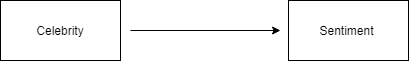
\includegraphics{figures/TwitterConceptualModel.png}

We can see that the sentiment of tweets related to different celebrity
is directly connected to the celebrity itself. Therefor the conceptual
model is very simple consisting of two variables, ``Celebrity'' and
``Sentiment''.

\subsubsection{Homogeneity of variance
analysis}\label{homogeneity-of-variance-analysis}

Analyze the homogeneity of variance of sentiments of the tweets of the
different celebrities

Lets start by looking at how the boxplot looks for each person and the
relevant sentiment that has been analysed.

\begin{Shaded}
\begin{Highlighting}[]
\CommentTok{#this was not here in the intermediate report.}
\CommentTok{#include your code and output in the document}
\KeywordTok{boxplot}\NormalTok{(score }\OperatorTok{~}\StringTok{ }\NormalTok{Person, }\DataTypeTok{data=}\NormalTok{semFrame, }\DataTypeTok{main=}\StringTok{"Boxplot of sentiment for each person"}\NormalTok{,}
        \DataTypeTok{xlab=}\StringTok{"Person"}\NormalTok{, }\DataTypeTok{ylab=}\StringTok{"Sentiment"}\NormalTok{)}
\end{Highlighting}
\end{Shaded}

\includegraphics{Coursework_assignment_A-team_5_files/figure-latex/unnamed-chunk-2-1.pdf}

\begin{Shaded}
\begin{Highlighting}[]
\KeywordTok{leveneTest}\NormalTok{( semFrame}\OperatorTok{$}\NormalTok{score,semFrame}\OperatorTok{$}\NormalTok{Person, }\DataTypeTok{center =}\NormalTok{ median)}
\end{Highlighting}
\end{Shaded}

\begin{verbatim}
## Levene's Test for Homogeneity of Variance (center = median)
##         Df F value    Pr(>F)    
## group    2  9.0536 0.0001202 ***
##       2997                      
## ---
## Signif. codes:  0 '***' 0.001 '**' 0.01 '*' 0.05 '.' 0.1 ' ' 1
\end{verbatim}

The Levene test results in a very low p-value., therefore the hypothesis
of equal variances is rejected and it is concluded that there is a
difference between the variances in the pipulation. Therefore the
variance is not considered to be homogeneous. \#\#\# Visual inspection
Graphically examine the variation in tweets' sentiments for each
celebrity (e.g.~histogram, density plot)

\begin{Shaded}
\begin{Highlighting}[]
\CommentTok{#include your code and output in the document}
\KeywordTok{hist}\NormalTok{(subsetBeyonce}\OperatorTok{$}\NormalTok{score)}
\end{Highlighting}
\end{Shaded}

\includegraphics{Coursework_assignment_A-team_5_files/figure-latex/unnamed-chunk-3-1.pdf}

\begin{Shaded}
\begin{Highlighting}[]
\KeywordTok{hist}\NormalTok{(subsetMadonna}\OperatorTok{$}\NormalTok{score)}
\end{Highlighting}
\end{Shaded}

\includegraphics{Coursework_assignment_A-team_5_files/figure-latex/unnamed-chunk-3-2.pdf}

\begin{Shaded}
\begin{Highlighting}[]
\KeywordTok{hist}\NormalTok{(subsetWest}\OperatorTok{$}\NormalTok{score)}
\end{Highlighting}
\end{Shaded}

\includegraphics{Coursework_assignment_A-team_5_files/figure-latex/unnamed-chunk-3-3.pdf}

\subsubsection{Mean sentiments}\label{mean-sentiments}

Graphically examine the mean sentiments of tweets for each celebrity

Here below we plot the means of each class using plotmeans from the
package gplots.

\begin{Shaded}
\begin{Highlighting}[]
\KeywordTok{plotmeans}\NormalTok{(score }\OperatorTok{~}\StringTok{ }\NormalTok{Person, }\DataTypeTok{data =}\NormalTok{ semFrame,}\DataTypeTok{mean.labels =} \OtherTok{TRUE}\NormalTok{,}\DataTypeTok{connect =} \OtherTok{FALSE}\NormalTok{,}\DataTypeTok{ylim =} \KeywordTok{c}\NormalTok{(}\OperatorTok{-}\FloatTok{0.1}\NormalTok{,}\FloatTok{0.8}\NormalTok{))}
\end{Highlighting}
\end{Shaded}

\includegraphics{Coursework_assignment_A-team_5_files/figure-latex/unnamed-chunk-4-1.pdf}

\subsubsection{Linear model}\label{linear-model}

\begin{Shaded}
\begin{Highlighting}[]
\CommentTok{#include your code and output in the document}
\NormalTok{ model0<-}\StringTok{ }\KeywordTok{lm}\NormalTok{(score }\OperatorTok{~}\StringTok{ }\DecValTok{1}\NormalTok{, }\DataTypeTok{data =}\NormalTok{ semFrame) }\CommentTok{#model without predictor}
\NormalTok{ model1<-}\StringTok{ }\KeywordTok{lm}\NormalTok{(score }\OperatorTok{~}\StringTok{ }\NormalTok{Person, }\DataTypeTok{data =}\NormalTok{ semFrame) }\CommentTok{#model with predictor}
\NormalTok{ AnovaResults <-}\KeywordTok{anova}\NormalTok{(model0,model1)}
\end{Highlighting}
\end{Shaded}

\emph{AnovaResults\$\texttt{Pr(\textgreater{}F)}{[}2{]}} For example if
the F(2,2997) is 3.74(for one example dataset) and the p = 0.024. That
means the sentiment of tweets is significantly different depending on
what celebrity is mentioned in the tweet.

Other results can be interpreted in the same manner.

\subsubsection{Post Hoc analysis}\label{post-hoc-analysis}

If a model that includes the celebrity is better in explaining the
sentiments of tweets than a model without such predictor, conduct a
post-hoc analysis with e.g.~Bonferroni correction, to examine which of
celebrity tweets differ from the other celebrity tweets

\begin{Shaded}
\begin{Highlighting}[]
\CommentTok{#include your code and output in the document}
\KeywordTok{pairwise.t.test}\NormalTok{(semFrame}\OperatorTok{$}\NormalTok{score, semFrame}\OperatorTok{$}\NormalTok{Person, }\DataTypeTok{paired =} \OtherTok{FALSE}\NormalTok{, }\DataTypeTok{p.adjust.method =} \StringTok{"bonferroni"}\NormalTok{)}
\end{Highlighting}
\end{Shaded}

\begin{verbatim}
## 
##  Pairwise comparisons using t tests with pooled SD 
## 
## data:  semFrame$score and semFrame$Person 
## 
##         Beyonce Madonna
## Madonna 1       -      
## West    1.6e-09 8.0e-12
## 
## P value adjustment method: bonferroni
\end{verbatim}

We chose to use the Bonferroni method to conduct this post-hoc analysis.
There the p-values are multiplied bu the number of comparisons.

I will include the results from a former run and analyse those results.
The results from the current run can than be interpreted the same way.

We will analyse these results when Beyonce vs Madonna : 1.2e-14 Beyonce
vs West : 7.5e-05 Madonna vs West : \textless{} 2e-16

According to results here above: Madonna vs West has significance that
is adjusted to bonferroni of 1.2 e-14, the value can be read in the same
manner for the other pairs.So since Beyonce and West have the highest
value, they have the lowest significance. And the Tweets for Madonna and
West differ the most since they have the lowest p-value.

\subsubsection{Report section for a scientific
publication}\label{report-section-for-a-scientific-publication}

Note that since the most recent Tweets are gathered each time we run the
markdown file, the exact numbers of our analysis will change a bit each
time.So some assumptions might be a bit distorted.

A linear model was fitted on the number of the sentiment score,
comparing the difference when taking the relative celbrity in account
and not. According to the analysis we have seen that the sentiment of
Tweets is significantly correlated to the celebrity. Then A Post Hoc
analysis by the meas of Bonferroni was conducted. That resulted in the
fact that the tweets for West and Madonna differ the most. That can be
confirmed by looking at the visualizasion of the means of the tweet
sentiment per person.

\subsection{Question 2 - Website visits (between groups - Two
factors)}\label{question-2---website-visits-between-groups---two-factors}

\subsubsection{Conceptual model}\label{conceptual-model-1}

The model can be found in the figure below.
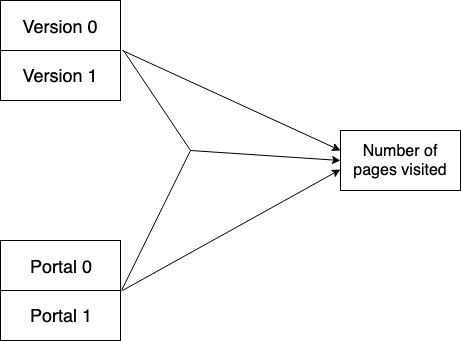
\includegraphics[width=0.50000\textwidth]{figures/Model_Question_2.png}

\subsubsection{Visual inspection}\label{visual-inspection}

Graphically examine the variation in page visits for different factors
levels (e.g.~histogram, density plot etc.)

\begin{Shaded}
\begin{Highlighting}[]
\NormalTok{myData <-}\StringTok{ }\KeywordTok{read.csv}\NormalTok{(}\StringTok{"webvisita.csv"}\NormalTok{,}\DataTypeTok{header=}\OtherTok{TRUE}\NormalTok{)}
\CommentTok{# We transform into factors what need to be.}
\NormalTok{myData}\OperatorTok{$}\NormalTok{user <-}\StringTok{ }\KeywordTok{factor}\NormalTok{(myData}\OperatorTok{$}\NormalTok{user)}
\NormalTok{myData}\OperatorTok{$}\NormalTok{version <-}\StringTok{ }\KeywordTok{factor}\NormalTok{(myData}\OperatorTok{$}\NormalTok{version, }\DataTypeTok{levels=}\KeywordTok{c}\NormalTok{(}\DecValTok{0}\OperatorTok{:}\DecValTok{1}\NormalTok{), }\DataTypeTok{labels=}\KeywordTok{c}\NormalTok{(}\StringTok{"old"}\NormalTok{,}\StringTok{"new"}\NormalTok{))}
\NormalTok{myData}\OperatorTok{$}\NormalTok{portal <-}\StringTok{ }\KeywordTok{factor}\NormalTok{(myData}\OperatorTok{$}\NormalTok{portal, }\DataTypeTok{levels=}\KeywordTok{c}\NormalTok{(}\DecValTok{0}\OperatorTok{:}\DecValTok{1}\NormalTok{),}\DataTypeTok{labels=}\KeywordTok{c}\NormalTok{(}\StringTok{"consummer"}\NormalTok{,}\StringTok{"company"}\NormalTok{))}

\KeywordTok{hist}\NormalTok{(myData}\OperatorTok{$}\NormalTok{pages, }\DataTypeTok{xlab=}\StringTok{"Number of pages visited"}\NormalTok{, }\DataTypeTok{main =} \StringTok{"Histogram of the number of pages visited"}\NormalTok{)}
\end{Highlighting}
\end{Shaded}

\includegraphics{Coursework_assignment_A-team_5_files/figure-latex/unnamed-chunk-7-1.pdf}

\begin{Shaded}
\begin{Highlighting}[]
\KeywordTok{plot}\NormalTok{(}\KeywordTok{density}\NormalTok{(myData}\OperatorTok{$}\NormalTok{pages), }\DataTypeTok{xlab=}\StringTok{"Number of pages visited"}\NormalTok{, }\DataTypeTok{main =} \StringTok{"density of the number of pages visited"}\NormalTok{)}
\end{Highlighting}
\end{Shaded}

\includegraphics{Coursework_assignment_A-team_5_files/figure-latex/unnamed-chunk-7-2.pdf}

\subsubsection{Normality check}\label{normality-check}

Statistically test if variable page visits deviates from normal
distribution

We can see that the data does not seems to come from a normal
distribution, thus we will do a normality test.

\begin{Shaded}
\begin{Highlighting}[]
\KeywordTok{shapiro.test}\NormalTok{(myData}\OperatorTok{$}\NormalTok{pages)}
\end{Highlighting}
\end{Shaded}

\begin{verbatim}
## 
##  Shapiro-Wilk normality test
## 
## data:  myData$pages
## W = 0.8436, p-value < 2.2e-16
\end{verbatim}

The really small p-value indcates here that there is a high probability
that this data do not come from a normal distribution.

\subsubsection{Model analysis}\label{model-analysis}

Conduct a model analysis, to examine the added values of adding 2
factors and interaction between the factors in the model to predict page
visits.

\begin{Shaded}
\begin{Highlighting}[]
\KeywordTok{library}\NormalTok{(pander)}
\CommentTok{# We create all the different models}
\NormalTok{model0 <-}\StringTok{ }\KeywordTok{lm}\NormalTok{(pages }\OperatorTok{~}\StringTok{ }\DecValTok{1}\NormalTok{, }\DataTypeTok{data=}\NormalTok{myData)}
\NormalTok{model1 <-}\StringTok{ }\KeywordTok{lm}\NormalTok{(pages }\OperatorTok{~}\StringTok{ }\NormalTok{version, }\DataTypeTok{data=}\NormalTok{myData)}
\NormalTok{model2 <-}\StringTok{ }\KeywordTok{lm}\NormalTok{(pages }\OperatorTok{~}\StringTok{ }\NormalTok{portal, }\DataTypeTok{data=}\NormalTok{myData)}
\NormalTok{model3 <-}\StringTok{ }\KeywordTok{lm}\NormalTok{(pages }\OperatorTok{~}\StringTok{ }\NormalTok{version }\OperatorTok{+}\StringTok{ }\NormalTok{portal, }\DataTypeTok{data=}\NormalTok{myData)}
\NormalTok{model4 <-}\StringTok{ }\KeywordTok{lm}\NormalTok{(pages }\OperatorTok{~}\StringTok{ }\NormalTok{version }\OperatorTok{+}\StringTok{ }\NormalTok{portal }\OperatorTok{+}\StringTok{ }\NormalTok{version}\OperatorTok{:}\NormalTok{portal, }\DataTypeTok{data =}\NormalTok{ myData)}


\KeywordTok{pander}\NormalTok{(}\KeywordTok{anova}\NormalTok{(model0,model1,}\DataTypeTok{test=}\StringTok{"F"}\NormalTok{),}\DataTypeTok{caption =} \StringTok{"Version as main effect on the number of pages visited"}\NormalTok{)}
\end{Highlighting}
\end{Shaded}

\begin{longtable}[]{@{}cccccc@{}}
\caption{Version as main effect on the number of pages
visited}\tabularnewline
\toprule
\begin{minipage}[b]{0.10\columnwidth}\centering\strut
Res.Df\strut
\end{minipage} & \begin{minipage}[b]{0.08\columnwidth}\centering\strut
RSS\strut
\end{minipage} & \begin{minipage}[b]{0.06\columnwidth}\centering\strut
Df\strut
\end{minipage} & \begin{minipage}[b]{0.14\columnwidth}\centering\strut
Sum of Sq\strut
\end{minipage} & \begin{minipage}[b]{0.08\columnwidth}\centering\strut
F\strut
\end{minipage} & \begin{minipage}[b]{0.12\columnwidth}\centering\strut
Pr(\textgreater{}F)\strut
\end{minipage}\tabularnewline
\midrule
\endfirsthead
\toprule
\begin{minipage}[b]{0.10\columnwidth}\centering\strut
Res.Df\strut
\end{minipage} & \begin{minipage}[b]{0.08\columnwidth}\centering\strut
RSS\strut
\end{minipage} & \begin{minipage}[b]{0.06\columnwidth}\centering\strut
Df\strut
\end{minipage} & \begin{minipage}[b]{0.14\columnwidth}\centering\strut
Sum of Sq\strut
\end{minipage} & \begin{minipage}[b]{0.08\columnwidth}\centering\strut
F\strut
\end{minipage} & \begin{minipage}[b]{0.12\columnwidth}\centering\strut
Pr(\textgreater{}F)\strut
\end{minipage}\tabularnewline
\midrule
\endhead
\begin{minipage}[t]{0.10\columnwidth}\centering\strut
998\strut
\end{minipage} & \begin{minipage}[t]{0.08\columnwidth}\centering\strut
2858\strut
\end{minipage} & \begin{minipage}[t]{0.06\columnwidth}\centering\strut
NA\strut
\end{minipage} & \begin{minipage}[t]{0.14\columnwidth}\centering\strut
NA\strut
\end{minipage} & \begin{minipage}[t]{0.08\columnwidth}\centering\strut
NA\strut
\end{minipage} & \begin{minipage}[t]{0.12\columnwidth}\centering\strut
NA\strut
\end{minipage}\tabularnewline
\begin{minipage}[t]{0.10\columnwidth}\centering\strut
997\strut
\end{minipage} & \begin{minipage}[t]{0.08\columnwidth}\centering\strut
2838\strut
\end{minipage} & \begin{minipage}[t]{0.06\columnwidth}\centering\strut
1\strut
\end{minipage} & \begin{minipage}[t]{0.14\columnwidth}\centering\strut
19.9\strut
\end{minipage} & \begin{minipage}[t]{0.08\columnwidth}\centering\strut
6.99\strut
\end{minipage} & \begin{minipage}[t]{0.12\columnwidth}\centering\strut
0.008324\strut
\end{minipage}\tabularnewline
\bottomrule
\end{longtable}

\begin{Shaded}
\begin{Highlighting}[]
\KeywordTok{pander}\NormalTok{(}\KeywordTok{anova}\NormalTok{(model0,model2,}\DataTypeTok{test=}\StringTok{"F"}\NormalTok{),}\DataTypeTok{caption =} \StringTok{"Portal as main effect on the number of pages visited"}\NormalTok{)}
\end{Highlighting}
\end{Shaded}

\begin{longtable}[]{@{}cccccc@{}}
\caption{Portal as main effect on the number of pages
visited}\tabularnewline
\toprule
\begin{minipage}[b]{0.10\columnwidth}\centering\strut
Res.Df\strut
\end{minipage} & \begin{minipage}[b]{0.08\columnwidth}\centering\strut
RSS\strut
\end{minipage} & \begin{minipage}[b]{0.06\columnwidth}\centering\strut
Df\strut
\end{minipage} & \begin{minipage}[b]{0.14\columnwidth}\centering\strut
Sum of Sq\strut
\end{minipage} & \begin{minipage}[b]{0.09\columnwidth}\centering\strut
F\strut
\end{minipage} & \begin{minipage}[b]{0.13\columnwidth}\centering\strut
Pr(\textgreater{}F)\strut
\end{minipage}\tabularnewline
\midrule
\endfirsthead
\toprule
\begin{minipage}[b]{0.10\columnwidth}\centering\strut
Res.Df\strut
\end{minipage} & \begin{minipage}[b]{0.08\columnwidth}\centering\strut
RSS\strut
\end{minipage} & \begin{minipage}[b]{0.06\columnwidth}\centering\strut
Df\strut
\end{minipage} & \begin{minipage}[b]{0.14\columnwidth}\centering\strut
Sum of Sq\strut
\end{minipage} & \begin{minipage}[b]{0.09\columnwidth}\centering\strut
F\strut
\end{minipage} & \begin{minipage}[b]{0.13\columnwidth}\centering\strut
Pr(\textgreater{}F)\strut
\end{minipage}\tabularnewline
\midrule
\endhead
\begin{minipage}[t]{0.10\columnwidth}\centering\strut
998\strut
\end{minipage} & \begin{minipage}[t]{0.08\columnwidth}\centering\strut
2858\strut
\end{minipage} & \begin{minipage}[t]{0.06\columnwidth}\centering\strut
NA\strut
\end{minipage} & \begin{minipage}[t]{0.14\columnwidth}\centering\strut
NA\strut
\end{minipage} & \begin{minipage}[t]{0.09\columnwidth}\centering\strut
NA\strut
\end{minipage} & \begin{minipage}[t]{0.13\columnwidth}\centering\strut
NA\strut
\end{minipage}\tabularnewline
\begin{minipage}[t]{0.10\columnwidth}\centering\strut
997\strut
\end{minipage} & \begin{minipage}[t]{0.08\columnwidth}\centering\strut
2695\strut
\end{minipage} & \begin{minipage}[t]{0.06\columnwidth}\centering\strut
1\strut
\end{minipage} & \begin{minipage}[t]{0.14\columnwidth}\centering\strut
162.9\strut
\end{minipage} & \begin{minipage}[t]{0.09\columnwidth}\centering\strut
60.28\strut
\end{minipage} & \begin{minipage}[t]{0.13\columnwidth}\centering\strut
2.033e-14\strut
\end{minipage}\tabularnewline
\bottomrule
\end{longtable}

\begin{Shaded}
\begin{Highlighting}[]
\KeywordTok{pander}\NormalTok{(}\KeywordTok{anova}\NormalTok{(model3,model4,}\DataTypeTok{test=}\StringTok{"F"}\NormalTok{),}\DataTypeTok{caption =} \StringTok{"Interaction effect on top of the two main effect"}\NormalTok{)}
\end{Highlighting}
\end{Shaded}

\begin{longtable}[]{@{}cccccc@{}}
\caption{Interaction effect on top of the two main
effect}\tabularnewline
\toprule
\begin{minipage}[b]{0.10\columnwidth}\centering\strut
Res.Df\strut
\end{minipage} & \begin{minipage}[b]{0.08\columnwidth}\centering\strut
RSS\strut
\end{minipage} & \begin{minipage}[b]{0.06\columnwidth}\centering\strut
Df\strut
\end{minipage} & \begin{minipage}[b]{0.14\columnwidth}\centering\strut
Sum of Sq\strut
\end{minipage} & \begin{minipage}[b]{0.09\columnwidth}\centering\strut
F\strut
\end{minipage} & \begin{minipage}[b]{0.13\columnwidth}\centering\strut
Pr(\textgreater{}F)\strut
\end{minipage}\tabularnewline
\midrule
\endfirsthead
\toprule
\begin{minipage}[b]{0.10\columnwidth}\centering\strut
Res.Df\strut
\end{minipage} & \begin{minipage}[b]{0.08\columnwidth}\centering\strut
RSS\strut
\end{minipage} & \begin{minipage}[b]{0.06\columnwidth}\centering\strut
Df\strut
\end{minipage} & \begin{minipage}[b]{0.14\columnwidth}\centering\strut
Sum of Sq\strut
\end{minipage} & \begin{minipage}[b]{0.09\columnwidth}\centering\strut
F\strut
\end{minipage} & \begin{minipage}[b]{0.13\columnwidth}\centering\strut
Pr(\textgreater{}F)\strut
\end{minipage}\tabularnewline
\midrule
\endhead
\begin{minipage}[t]{0.10\columnwidth}\centering\strut
996\strut
\end{minipage} & \begin{minipage}[t]{0.08\columnwidth}\centering\strut
2679\strut
\end{minipage} & \begin{minipage}[t]{0.06\columnwidth}\centering\strut
NA\strut
\end{minipage} & \begin{minipage}[t]{0.14\columnwidth}\centering\strut
NA\strut
\end{minipage} & \begin{minipage}[t]{0.09\columnwidth}\centering\strut
NA\strut
\end{minipage} & \begin{minipage}[t]{0.13\columnwidth}\centering\strut
NA\strut
\end{minipage}\tabularnewline
\begin{minipage}[t]{0.10\columnwidth}\centering\strut
995\strut
\end{minipage} & \begin{minipage}[t]{0.08\columnwidth}\centering\strut
2593\strut
\end{minipage} & \begin{minipage}[t]{0.06\columnwidth}\centering\strut
1\strut
\end{minipage} & \begin{minipage}[t]{0.14\columnwidth}\centering\strut
86.47\strut
\end{minipage} & \begin{minipage}[t]{0.09\columnwidth}\centering\strut
33.18\strut
\end{minipage} & \begin{minipage}[t]{0.13\columnwidth}\centering\strut
1.118e-08\strut
\end{minipage}\tabularnewline
\bottomrule
\end{longtable}

\begin{Shaded}
\begin{Highlighting}[]
\KeywordTok{pander}\NormalTok{(}\KeywordTok{anova}\NormalTok{(model4),}\DataTypeTok{caption =} \StringTok{"Effect of version, portal and interaction effect on the number of pages visited"}\NormalTok{)}
\end{Highlighting}
\end{Shaded}

\begin{longtable}[]{@{}cccccc@{}}
\caption{Effect of version, portal and interaction effect on the number
of pages visited}\tabularnewline
\toprule
\begin{minipage}[b]{0.24\columnwidth}\centering\strut
~\strut
\end{minipage} & \begin{minipage}[b]{0.07\columnwidth}\centering\strut
Df\strut
\end{minipage} & \begin{minipage}[b]{0.10\columnwidth}\centering\strut
Sum Sq\strut
\end{minipage} & \begin{minipage}[b]{0.12\columnwidth}\centering\strut
Mean Sq\strut
\end{minipage} & \begin{minipage}[b]{0.12\columnwidth}\centering\strut
F value\strut
\end{minipage} & \begin{minipage}[b]{0.13\columnwidth}\centering\strut
Pr(\textgreater{}F)\strut
\end{minipage}\tabularnewline
\midrule
\endfirsthead
\toprule
\begin{minipage}[b]{0.24\columnwidth}\centering\strut
~\strut
\end{minipage} & \begin{minipage}[b]{0.07\columnwidth}\centering\strut
Df\strut
\end{minipage} & \begin{minipage}[b]{0.10\columnwidth}\centering\strut
Sum Sq\strut
\end{minipage} & \begin{minipage}[b]{0.12\columnwidth}\centering\strut
Mean Sq\strut
\end{minipage} & \begin{minipage}[b]{0.12\columnwidth}\centering\strut
F value\strut
\end{minipage} & \begin{minipage}[b]{0.13\columnwidth}\centering\strut
Pr(\textgreater{}F)\strut
\end{minipage}\tabularnewline
\midrule
\endhead
\begin{minipage}[t]{0.24\columnwidth}\centering\strut
\textbf{version}\strut
\end{minipage} & \begin{minipage}[t]{0.07\columnwidth}\centering\strut
1\strut
\end{minipage} & \begin{minipage}[t]{0.10\columnwidth}\centering\strut
19.9\strut
\end{minipage} & \begin{minipage}[t]{0.12\columnwidth}\centering\strut
19.9\strut
\end{minipage} & \begin{minipage}[t]{0.12\columnwidth}\centering\strut
7.636\strut
\end{minipage} & \begin{minipage}[t]{0.13\columnwidth}\centering\strut
0.005828\strut
\end{minipage}\tabularnewline
\begin{minipage}[t]{0.24\columnwidth}\centering\strut
\textbf{portal}\strut
\end{minipage} & \begin{minipage}[t]{0.07\columnwidth}\centering\strut
1\strut
\end{minipage} & \begin{minipage}[t]{0.10\columnwidth}\centering\strut
158.6\strut
\end{minipage} & \begin{minipage}[t]{0.12\columnwidth}\centering\strut
158.6\strut
\end{minipage} & \begin{minipage}[t]{0.12\columnwidth}\centering\strut
60.86\strut
\end{minipage} & \begin{minipage}[t]{0.13\columnwidth}\centering\strut
1.546e-14\strut
\end{minipage}\tabularnewline
\begin{minipage}[t]{0.24\columnwidth}\centering\strut
\textbf{version:portal}\strut
\end{minipage} & \begin{minipage}[t]{0.07\columnwidth}\centering\strut
1\strut
\end{minipage} & \begin{minipage}[t]{0.10\columnwidth}\centering\strut
86.47\strut
\end{minipage} & \begin{minipage}[t]{0.12\columnwidth}\centering\strut
86.47\strut
\end{minipage} & \begin{minipage}[t]{0.12\columnwidth}\centering\strut
33.18\strut
\end{minipage} & \begin{minipage}[t]{0.13\columnwidth}\centering\strut
1.118e-08\strut
\end{minipage}\tabularnewline
\begin{minipage}[t]{0.24\columnwidth}\centering\strut
\textbf{Residuals}\strut
\end{minipage} & \begin{minipage}[t]{0.07\columnwidth}\centering\strut
995\strut
\end{minipage} & \begin{minipage}[t]{0.10\columnwidth}\centering\strut
2593\strut
\end{minipage} & \begin{minipage}[t]{0.12\columnwidth}\centering\strut
2.606\strut
\end{minipage} & \begin{minipage}[t]{0.12\columnwidth}\centering\strut
NA\strut
\end{minipage} & \begin{minipage}[t]{0.13\columnwidth}\centering\strut
NA\strut
\end{minipage}\tabularnewline
\bottomrule
\end{longtable}

We see a significant two-way interaction effect, we will thus perform a
simple effect analysis to better understand this interaction effect.

\subsubsection{Simple effect analysis}\label{simple-effect-analysis}

If the analysis shows a significant two-way interaction effect, conduct
a Simple Effect analysis to explore this interaction effect in more
detail.It helps first to look at the means in a figure

\begin{Shaded}
\begin{Highlighting}[]
\NormalTok{myData}\OperatorTok{$}\NormalTok{simple <-}\StringTok{ }\KeywordTok{interaction}\NormalTok{(myData}\OperatorTok{$}\NormalTok{version, myData}\OperatorTok{$}\NormalTok{portal) }\CommentTok{#merge two factors }

\NormalTok{contrastConsummer <-}\KeywordTok{c}\NormalTok{(}\DecValTok{1}\NormalTok{,}\OperatorTok{-}\DecValTok{1}\NormalTok{,}\DecValTok{0}\NormalTok{,}\DecValTok{0}\NormalTok{) }\CommentTok{#Only the consummer portal data }
\NormalTok{contrastCompany <-}\KeywordTok{c}\NormalTok{(}\DecValTok{0}\NormalTok{,}\DecValTok{0}\NormalTok{,}\DecValTok{1}\NormalTok{,}\OperatorTok{-}\DecValTok{1}\NormalTok{) }\CommentTok{#Only the company portal data }

\NormalTok{SimpleEff <-}\StringTok{ }\KeywordTok{cbind}\NormalTok{(contrastConsummer,contrastCompany)}
\KeywordTok{contrasts}\NormalTok{(myData}\OperatorTok{$}\NormalTok{simple) <-}\StringTok{ }\NormalTok{SimpleEff }\CommentTok{#now we link the two contrasts with the factor simple}
\KeywordTok{pander}\NormalTok{(simpleEffectModel <-}\KeywordTok{lm}\NormalTok{(pages }\OperatorTok{~}\StringTok{ }\NormalTok{simple , }\DataTypeTok{data =}\NormalTok{ myData, }\DataTypeTok{na.action =}\NormalTok{ na.exclude), }\DataTypeTok{caption =} \StringTok{"Simple effect analysis"}\NormalTok{)}
\end{Highlighting}
\end{Shaded}

\begin{longtable}[]{@{}ccccc@{}}
\caption{Simple effect analysis}\tabularnewline
\toprule
\begin{minipage}[b]{0.34\columnwidth}\centering\strut
~\strut
\end{minipage} & \begin{minipage}[b]{0.12\columnwidth}\centering\strut
Estimate\strut
\end{minipage} & \begin{minipage}[b]{0.15\columnwidth}\centering\strut
Std. Error\strut
\end{minipage} & \begin{minipage}[b]{0.11\columnwidth}\centering\strut
t value\strut
\end{minipage} & \begin{minipage}[b]{0.14\columnwidth}\centering\strut
Pr(\textgreater{}\textbar{}t\textbar{})\strut
\end{minipage}\tabularnewline
\midrule
\endfirsthead
\toprule
\begin{minipage}[b]{0.34\columnwidth}\centering\strut
~\strut
\end{minipage} & \begin{minipage}[b]{0.12\columnwidth}\centering\strut
Estimate\strut
\end{minipage} & \begin{minipage}[b]{0.15\columnwidth}\centering\strut
Std. Error\strut
\end{minipage} & \begin{minipage}[b]{0.11\columnwidth}\centering\strut
t value\strut
\end{minipage} & \begin{minipage}[b]{0.14\columnwidth}\centering\strut
Pr(\textgreater{}\textbar{}t\textbar{})\strut
\end{minipage}\tabularnewline
\midrule
\endhead
\begin{minipage}[t]{0.34\columnwidth}\centering\strut
\textbf{(Intercept)}\strut
\end{minipage} & \begin{minipage}[t]{0.12\columnwidth}\centering\strut
2.689\strut
\end{minipage} & \begin{minipage}[t]{0.15\columnwidth}\centering\strut
0.05118\strut
\end{minipage} & \begin{minipage}[t]{0.11\columnwidth}\centering\strut
52.54\strut
\end{minipage} & \begin{minipage}[t]{0.14\columnwidth}\centering\strut
2.964e-289\strut
\end{minipage}\tabularnewline
\begin{minipage}[t]{0.34\columnwidth}\centering\strut
\textbf{simplecontrastConsummer}\strut
\end{minipage} & \begin{minipage}[t]{0.12\columnwidth}\centering\strut
-0.1701\strut
\end{minipage} & \begin{minipage}[t]{0.15\columnwidth}\centering\strut
0.07241\strut
\end{minipage} & \begin{minipage}[t]{0.11\columnwidth}\centering\strut
-2.349\strut
\end{minipage} & \begin{minipage}[t]{0.14\columnwidth}\centering\strut
0.01904\strut
\end{minipage}\tabularnewline
\begin{minipage}[t]{0.34\columnwidth}\centering\strut
\textbf{simplecontrastCompany}\strut
\end{minipage} & \begin{minipage}[t]{0.12\columnwidth}\centering\strut
0.4196\strut
\end{minipage} & \begin{minipage}[t]{0.15\columnwidth}\centering\strut
0.07235\strut
\end{minipage} & \begin{minipage}[t]{0.11\columnwidth}\centering\strut
5.799\strut
\end{minipage} & \begin{minipage}[t]{0.14\columnwidth}\centering\strut
8.94e-09\strut
\end{minipage}\tabularnewline
\begin{minipage}[t]{0.34\columnwidth}\centering\strut
\textbf{simple}\strut
\end{minipage} & \begin{minipage}[t]{0.12\columnwidth}\centering\strut
0.7676\strut
\end{minipage} & \begin{minipage}[t]{0.15\columnwidth}\centering\strut
0.1024\strut
\end{minipage} & \begin{minipage}[t]{0.11\columnwidth}\centering\strut
7.498\strut
\end{minipage} & \begin{minipage}[t]{0.14\columnwidth}\centering\strut
1.428e-13\strut
\end{minipage}\tabularnewline
\bottomrule
\end{longtable}

\subsubsection{Report section for a scientific
publication}\label{report-section-for-a-scientific-publication-1}

Write a small section for a scientific publication, in which you report
the results of the analyses, and explain the conclusions that can be
drawn.

A linear model was fitted on the number of pages visited of a website,
taking the version of the website (an old version and a new one) and the
portal that was used to access the website (a portal for consumers and
one for companies) as independent variables, and including a two-way
interaction between these variables. The analysis found a significant
main effect for the version (F(1,995) = 7.6357, p. \textless{} 0.006)and
for the portal (F(1,995) = 60.8571, p. \textless{} 10\^{}-13). It also
found a significant two-way interaction effect ( F(1, 995) = 33.1827, p.
\textless{} 10\^{}-7) between these two variables. ((((However, since a
lot of data was used, one can put in doubt the significance result of
the version, especially compared to the F values of the portal and the
interaction between the variables.)))) The two-way interaction was
further examined by a Simple Effect analysis. It found a significant
difference for the version in the portal for consumer (t = -2.349, p. =
0.019) as well as in the portal for companies (t = 5.799, p. \textless{}
9e-09).

\subsection{Question 3 - Linear regression
analysis}\label{question-3---linear-regression-analysis}

\subsubsection{Conceptual model}\label{conceptual-model-2}

For this assignment we retrieved a data set from
\url{http://www.stat.ufl.edu/~winner/datasets.html}. The dataset
contains facts about 153 hybrid cars, including their price, year built,
acceleration data and fuel consumption; those are the four quantitative
variables that will be the subject of the linear model in this question.
We would like to predict the price of the car (response variable), using
data on acceleration rate of the car, the fuel consumption and the year
that it was built. The conceptual model for this research looks like
this:

\begin{figure}
\centering
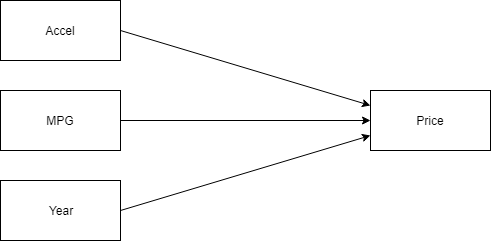
\includegraphics{figures/Conceptual_Model_Q3.png}
\caption{Conceptual model of the four considered variables}
\end{figure}

\subsubsection{Visual inspection}\label{visual-inspection-1}

The distribution of the independent variable is displayed

\begin{Shaded}
\begin{Highlighting}[]
\CommentTok{# Reading in the necessary packages}
\KeywordTok{library}\NormalTok{(readr)}
\NormalTok{d <-}\StringTok{ }\KeywordTok{read_csv}\NormalTok{(}\StringTok{"hybrid_reg.csv"}\NormalTok{)}
\NormalTok{mpg <-}\StringTok{ }\NormalTok{d}\OperatorTok{$}\NormalTok{mpg}
\NormalTok{year <-}\StringTok{ }\NormalTok{d}\OperatorTok{$}\NormalTok{year}
\NormalTok{accel <-}\StringTok{ }\NormalTok{d}\OperatorTok{$}\NormalTok{accelrate}
\NormalTok{price <-}\StringTok{ }\NormalTok{d}\OperatorTok{$}\NormalTok{msrp}

\CommentTok{# Histogram of the distribution of the price variable}
\KeywordTok{hist}\NormalTok{(price)}
\end{Highlighting}
\end{Shaded}

\includegraphics{Coursework_assignment_A-team_5_files/figure-latex/unnamed-chunk-11-1.pdf}

\begin{Shaded}
\begin{Highlighting}[]
\CommentTok{# Density plot of the price variable}
\KeywordTok{plot}\NormalTok{(}\KeywordTok{density}\NormalTok{(price),}\DataTypeTok{main=}\StringTok{"Density plot of price"}\NormalTok{)}
\end{Highlighting}
\end{Shaded}

\includegraphics{Coursework_assignment_A-team_5_files/figure-latex/unnamed-chunk-11-2.pdf}
Visual inspection of the plots reveals that the distribution of price
deviates from a normal distribution. Especially the right tail of the
density distribution has more mass than it should have. Since the
distribution is right skewed, a logarithmic transformation is effective
in increasing the normality; the result can be seen in the figure below.

\begin{Shaded}
\begin{Highlighting}[]
\CommentTok{# Density plot of the transformed price variable}
\KeywordTok{plot}\NormalTok{(}\KeywordTok{density}\NormalTok{(}\KeywordTok{log}\NormalTok{(price)),}\DataTypeTok{main=}\StringTok{"Density plot of log(price)"}\NormalTok{)}
\end{Highlighting}
\end{Shaded}

\includegraphics{Coursework_assignment_A-team_5_files/figure-latex/unnamed-chunk-12-1.pdf}

\begin{Shaded}
\begin{Highlighting}[]
\KeywordTok{shapiro.test}\NormalTok{(price)}
\end{Highlighting}
\end{Shaded}

\begin{verbatim}
## 
##  Shapiro-Wilk normality test
## 
## data:  price
## W = 0.85261, p-value = 4.345e-11
\end{verbatim}

\begin{Shaded}
\begin{Highlighting}[]
\KeywordTok{shapiro.test}\NormalTok{(}\KeywordTok{log}\NormalTok{(price))}
\end{Highlighting}
\end{Shaded}

\begin{verbatim}
## 
##  Shapiro-Wilk normality test
## 
## data:  log(price)
## W = 0.97322, p-value = 0.004424
\end{verbatim}

As we will see later on, the logarithmic transformation is also
necessary to justify the choice of linear regression, as without it the
assumptions for linear regression do not hold.

\subsubsection{Scatter plot}\label{scatter-plot}

Using scatter plots we can visually examine the relationship between two
variables. The following figures show the scatter plots of the response
variable price paired with each of the predictors.

\begin{Shaded}
\begin{Highlighting}[]
\KeywordTok{plot}\NormalTok{(}\KeywordTok{log}\NormalTok{(price) }\OperatorTok{~}\StringTok{ }\NormalTok{accel,}\DataTypeTok{main=}\StringTok{"log(price) vs accel"}\NormalTok{)}
\end{Highlighting}
\end{Shaded}

\includegraphics{Coursework_assignment_A-team_5_files/figure-latex/unnamed-chunk-13-1.pdf}

\begin{Shaded}
\begin{Highlighting}[]
\KeywordTok{plot}\NormalTok{(}\KeywordTok{log}\NormalTok{(price) }\OperatorTok{~}\StringTok{ }\NormalTok{mpg,}\DataTypeTok{main=}\StringTok{"log(price) vs mpg"}\NormalTok{)}
\end{Highlighting}
\end{Shaded}

\includegraphics{Coursework_assignment_A-team_5_files/figure-latex/unnamed-chunk-13-2.pdf}

\begin{Shaded}
\begin{Highlighting}[]
\KeywordTok{plot}\NormalTok{(}\KeywordTok{log}\NormalTok{(price) }\OperatorTok{~}\StringTok{ }\NormalTok{year,}\DataTypeTok{main=}\StringTok{"log(price) vs year"}\NormalTok{)}
\end{Highlighting}
\end{Shaded}

\includegraphics{Coursework_assignment_A-team_5_files/figure-latex/unnamed-chunk-13-3.pdf}

\subsubsection{Linear regression}\label{linear-regression}

From the anova table we can see that the accel and mpg variables are
able to significantly improve the model. The year variable is not able
to explain any additional significant variance in the price variable.
Therefore we exclude the price variable from further analysis.

\begin{Shaded}
\begin{Highlighting}[]
\KeywordTok{library}\NormalTok{(pander)}
\NormalTok{model0 <-}\StringTok{ }\KeywordTok{lm}\NormalTok{(}\KeywordTok{log}\NormalTok{(price) }\OperatorTok{~}\StringTok{ }\DecValTok{1}\NormalTok{)}
\NormalTok{model1 <-}\StringTok{ }\KeywordTok{lm}\NormalTok{(}\KeywordTok{log}\NormalTok{(price) }\OperatorTok{~}\StringTok{ }\NormalTok{accel)}
\NormalTok{model2 <-}\StringTok{ }\KeywordTok{lm}\NormalTok{(}\KeywordTok{log}\NormalTok{(price) }\OperatorTok{~}\StringTok{ }\NormalTok{accel }\OperatorTok{+}\StringTok{ }\NormalTok{mpg)}
\NormalTok{model3 <-}\StringTok{ }\KeywordTok{lm}\NormalTok{(}\KeywordTok{log}\NormalTok{(price) }\OperatorTok{~}\StringTok{ }\NormalTok{accel }\OperatorTok{+}\StringTok{ }\NormalTok{mpg }\OperatorTok{+}\StringTok{ }\NormalTok{year)}

\KeywordTok{pander}\NormalTok{(}\KeywordTok{anova}\NormalTok{(model0,model1,model2,model3), }
       \DataTypeTok{caption =} \StringTok{"Model comparison to predict the price of a car"}\NormalTok{)}
\end{Highlighting}
\end{Shaded}

\begin{longtable}[]{@{}cccccc@{}}
\caption{Model comparison to predict the price of a car}\tabularnewline
\toprule
\begin{minipage}[b]{0.10\columnwidth}\centering\strut
Res.Df\strut
\end{minipage} & \begin{minipage}[b]{0.09\columnwidth}\centering\strut
RSS\strut
\end{minipage} & \begin{minipage}[b]{0.06\columnwidth}\centering\strut
Df\strut
\end{minipage} & \begin{minipage}[b]{0.14\columnwidth}\centering\strut
Sum of Sq\strut
\end{minipage} & \begin{minipage}[b]{0.12\columnwidth}\centering\strut
F\strut
\end{minipage} & \begin{minipage}[b]{0.13\columnwidth}\centering\strut
Pr(\textgreater{}F)\strut
\end{minipage}\tabularnewline
\midrule
\endfirsthead
\toprule
\begin{minipage}[b]{0.10\columnwidth}\centering\strut
Res.Df\strut
\end{minipage} & \begin{minipage}[b]{0.09\columnwidth}\centering\strut
RSS\strut
\end{minipage} & \begin{minipage}[b]{0.06\columnwidth}\centering\strut
Df\strut
\end{minipage} & \begin{minipage}[b]{0.14\columnwidth}\centering\strut
Sum of Sq\strut
\end{minipage} & \begin{minipage}[b]{0.12\columnwidth}\centering\strut
F\strut
\end{minipage} & \begin{minipage}[b]{0.13\columnwidth}\centering\strut
Pr(\textgreater{}F)\strut
\end{minipage}\tabularnewline
\midrule
\endhead
\begin{minipage}[t]{0.10\columnwidth}\centering\strut
152\strut
\end{minipage} & \begin{minipage}[t]{0.09\columnwidth}\centering\strut
35.77\strut
\end{minipage} & \begin{minipage}[t]{0.06\columnwidth}\centering\strut
NA\strut
\end{minipage} & \begin{minipage}[t]{0.14\columnwidth}\centering\strut
NA\strut
\end{minipage} & \begin{minipage}[t]{0.12\columnwidth}\centering\strut
NA\strut
\end{minipage} & \begin{minipage}[t]{0.13\columnwidth}\centering\strut
NA\strut
\end{minipage}\tabularnewline
\begin{minipage}[t]{0.10\columnwidth}\centering\strut
151\strut
\end{minipage} & \begin{minipage}[t]{0.09\columnwidth}\centering\strut
18.83\strut
\end{minipage} & \begin{minipage}[t]{0.06\columnwidth}\centering\strut
1\strut
\end{minipage} & \begin{minipage}[t]{0.14\columnwidth}\centering\strut
16.94\strut
\end{minipage} & \begin{minipage}[t]{0.12\columnwidth}\centering\strut
146.9\strut
\end{minipage} & \begin{minipage}[t]{0.13\columnwidth}\centering\strut
5.776e-24\strut
\end{minipage}\tabularnewline
\begin{minipage}[t]{0.10\columnwidth}\centering\strut
150\strut
\end{minipage} & \begin{minipage}[t]{0.09\columnwidth}\centering\strut
17.19\strut
\end{minipage} & \begin{minipage}[t]{0.06\columnwidth}\centering\strut
1\strut
\end{minipage} & \begin{minipage}[t]{0.14\columnwidth}\centering\strut
1.639\strut
\end{minipage} & \begin{minipage}[t]{0.12\columnwidth}\centering\strut
14.22\strut
\end{minipage} & \begin{minipage}[t]{0.13\columnwidth}\centering\strut
0.0002343\strut
\end{minipage}\tabularnewline
\begin{minipage}[t]{0.10\columnwidth}\centering\strut
149\strut
\end{minipage} & \begin{minipage}[t]{0.09\columnwidth}\centering\strut
17.18\strut
\end{minipage} & \begin{minipage}[t]{0.06\columnwidth}\centering\strut
1\strut
\end{minipage} & \begin{minipage}[t]{0.14\columnwidth}\centering\strut
0.01013\strut
\end{minipage} & \begin{minipage}[t]{0.12\columnwidth}\centering\strut
0.08785\strut
\end{minipage} & \begin{minipage}[t]{0.13\columnwidth}\centering\strut
0.7673\strut
\end{minipage}\tabularnewline
\bottomrule
\end{longtable}

\begin{Shaded}
\begin{Highlighting}[]
\KeywordTok{library}\NormalTok{(QuantPsyc)}
\KeywordTok{pander}\NormalTok{(}\KeywordTok{confint}\NormalTok{(model2),}
       \DataTypeTok{caption =} \StringTok{"#95% confidence interval of the estimates"}\NormalTok{)}
\end{Highlighting}
\end{Shaded}

\begin{longtable}[]{@{}ccc@{}}
\caption{\#95\% confidence interval of the estimates}\tabularnewline
\toprule
\begin{minipage}[b]{0.23\columnwidth}\centering\strut
~\strut
\end{minipage} & \begin{minipage}[b]{0.13\columnwidth}\centering\strut
2.5 \%\strut
\end{minipage} & \begin{minipage}[b]{0.13\columnwidth}\centering\strut
97.5 \%\strut
\end{minipage}\tabularnewline
\midrule
\endfirsthead
\toprule
\begin{minipage}[b]{0.23\columnwidth}\centering\strut
~\strut
\end{minipage} & \begin{minipage}[b]{0.13\columnwidth}\centering\strut
2.5 \%\strut
\end{minipage} & \begin{minipage}[b]{0.13\columnwidth}\centering\strut
97.5 \%\strut
\end{minipage}\tabularnewline
\midrule
\endhead
\begin{minipage}[t]{0.23\columnwidth}\centering\strut
\textbf{(Intercept)}\strut
\end{minipage} & \begin{minipage}[t]{0.13\columnwidth}\centering\strut
9.328\strut
\end{minipage} & \begin{minipage}[t]{0.13\columnwidth}\centering\strut
10.13\strut
\end{minipage}\tabularnewline
\begin{minipage}[t]{0.23\columnwidth}\centering\strut
\textbf{accel}\strut
\end{minipage} & \begin{minipage}[t]{0.13\columnwidth}\centering\strut
0.07142\strut
\end{minipage} & \begin{minipage}[t]{0.13\columnwidth}\centering\strut
0.1142\strut
\end{minipage}\tabularnewline
\begin{minipage}[t]{0.23\columnwidth}\centering\strut
\textbf{mpg}\strut
\end{minipage} & \begin{minipage}[t]{0.13\columnwidth}\centering\strut
-0.0167\strut
\end{minipage} & \begin{minipage}[t]{0.13\columnwidth}\centering\strut
-0.00524\strut
\end{minipage}\tabularnewline
\bottomrule
\end{longtable}

\begin{Shaded}
\begin{Highlighting}[]
\KeywordTok{pander}\NormalTok{(}\KeywordTok{lm.beta}\NormalTok{(model2),}
       \DataTypeTok{caption =} \StringTok{"standardised regression coefficients"}\NormalTok{) }\CommentTok{# standardised regression coefficients}
\end{Highlighting}
\end{Shaded}

\begin{longtable}[]{@{}cc@{}}
\toprule
\begin{minipage}[b]{0.12\columnwidth}\centering\strut
accel\strut
\end{minipage} & \begin{minipage}[b]{0.12\columnwidth}\centering\strut
mpg\strut
\end{minipage}\tabularnewline
\midrule
\endhead
\begin{minipage}[t]{0.12\columnwidth}\centering\strut
0.5626\strut
\end{minipage} & \begin{minipage}[t]{0.12\columnwidth}\centering\strut
-0.2482\strut
\end{minipage}\tabularnewline
\bottomrule
\end{longtable}

\subsubsection{Examine assumption}\label{examine-assumption}

The residuals vs fitted plot is a useful tool in examining the linearity
and equal variances assumptions.

\begin{Shaded}
\begin{Highlighting}[]
\NormalTok{residuals =}\StringTok{ }\KeywordTok{resid}\NormalTok{(model2)}
\KeywordTok{plot}\NormalTok{(residuals }\OperatorTok{~}\StringTok{ }\KeywordTok{fitted}\NormalTok{(model2))}
\end{Highlighting}
\end{Shaded}

\includegraphics{Coursework_assignment_A-team_5_files/figure-latex/unnamed-chunk-16-1.pdf}
For normality we can check the qq-plot:

\begin{Shaded}
\begin{Highlighting}[]
\KeywordTok{library}\NormalTok{(car)}
\KeywordTok{qqnorm}\NormalTok{(residuals)}
\KeywordTok{qqline}\NormalTok{(residuals)}
\end{Highlighting}
\end{Shaded}

\includegraphics{Coursework_assignment_A-team_5_files/figure-latex/unnamed-chunk-17-1.pdf}
Multicollinearity:

\begin{Shaded}
\begin{Highlighting}[]
\KeywordTok{vif}\NormalTok{(model2)}
\end{Highlighting}
\end{Shaded}

\begin{verbatim}
##   accel     mpg 
## 1.34428 1.34428
\end{verbatim}

\begin{Shaded}
\begin{Highlighting}[]
\DecValTok{1}\OperatorTok{/}\KeywordTok{vif}\NormalTok{(model2) }\CommentTok{# Tolerance}
\end{Highlighting}
\end{Shaded}

\begin{verbatim}
##     accel       mpg 
## 0.7438928 0.7438928
\end{verbatim}

Autocorrelation:

\begin{Shaded}
\begin{Highlighting}[]
\KeywordTok{durbinWatsonTest}\NormalTok{(model2)}
\end{Highlighting}
\end{Shaded}

\begin{verbatim}
##  lag Autocorrelation D-W Statistic p-value
##    1       0.2303107      1.535374   0.006
##  Alternative hypothesis: rho != 0
\end{verbatim}

\subsubsection{Impact analysis of individual
cases}\label{impact-analysis-of-individual-cases}

\begin{Shaded}
\begin{Highlighting}[]
\NormalTok{d}\OperatorTok{$}\NormalTok{stud.res<-}\KeywordTok{rstudent}\NormalTok{(model2)}
\KeywordTok{plot}\NormalTok{(d}\OperatorTok{$}\NormalTok{stud.res)}
\end{Highlighting}
\end{Shaded}

\includegraphics{Coursework_assignment_A-team_5_files/figure-latex/unnamed-chunk-20-1.pdf}

\begin{Shaded}
\begin{Highlighting}[]
\NormalTok{d}\OperatorTok{$}\NormalTok{leverage<-}\KeywordTok{hatvalues}\NormalTok{(model2)}
\KeywordTok{plot}\NormalTok{(d}\OperatorTok{$}\NormalTok{leverage)}
\end{Highlighting}
\end{Shaded}

\includegraphics{Coursework_assignment_A-team_5_files/figure-latex/unnamed-chunk-20-2.pdf}

\begin{Shaded}
\begin{Highlighting}[]
\NormalTok{d}\OperatorTok{$}\NormalTok{cooks<-}\KeywordTok{cooks.distance}\NormalTok{(model2)}
\KeywordTok{plot}\NormalTok{(d}\OperatorTok{$}\NormalTok{cooks)}
\end{Highlighting}
\end{Shaded}

\includegraphics{Coursework_assignment_A-team_5_files/figure-latex/unnamed-chunk-20-3.pdf}

\subsubsection{Report section for a scientific
publication}\label{report-section-for-a-scientific-publication-2}

In this section we briefly present the results of fitting a linear
regression model in order to predict the price of cars using data on
their acceleration rate, their fuel efficiency in miles per gallon, and
their build year.

First of all we can conclude that a logarithmic transformation was
necessary to increase normality of the distribution of the price
variable. While the distribution still significantly differs from a
normal one (W = 0.973, p = 0.004), it is an improvement over the
original distribution (W = 0.853, p = 4.3e-11). Furthermore, the
transformation was necessary to justify the choice of performing linear
regression, as without it the assumptions for linear regression do not
hold, especially the linearity assumption.

Inspecting the scatter plots, it becomes clear that a linear
relationschip between the natural logarithm of price and the year the
car was built is absent. The scatter plots of the other two variables
show some indication that a relationship might exist.

Fitting the model revealed that the year variable is indeed not able to
explain any additional variance in the price variable on top of the
accel and mpg variables (F = 0.088, p = 0.77). Based on this result we
decided to exclude the independent variable year from the model. Hence
we end up with the following model:

log(price) = 9.73 + 0.093 x accel - 0.011 x mpg

Checking the assumptions of the linear regression, we found that the
distribution of the residuals is normal with expected value 0 and
(roughly) constant variance. Testing for independence showed a violation
of the assumption (D-W = 1.54, p = 0.008). Violating the independence
assumption is quite problematic, but for the sake of the exercise we
will continue the analysis. Additionally, no multicollinearity could be
found in our model.

Analysis of influential and leverage points revealed no severe outlying
cases that undermine the linear regression model.

The interpretation of the coefficients is slightly tricky, since we are
dealing with a transformed dependent variable. Instead of additive, the
model becomes multiplicative, and each coefficients has to be
interpreted as an exponent (i.e.~the intercept becomes e\^{}9.73 =
16,815). The standardized coefficients tell us that the effect of one
higher standard deviation in the acceleration rate has about twice the
effect on the price of one higher standard deviation in the fuel
efficiency.

To conclude, we were able to formulate a linear model that is to some
extent able to predict the price of a car based on its acceleration rate
and its fuel efficiency. Since not all assumptions of linear regression
were met, interpretation of the results requires caution.

\subsection{Question 4 - Logistic regression
analysis}\label{question-4---logistic-regression-analysis}

\begin{Shaded}
\begin{Highlighting}[]
\CommentTok{#include your code and output in the document}
\NormalTok{Data <-}\StringTok{ }\KeywordTok{read.csv}\NormalTok{(}\StringTok{"port_taiwan.csv"}\NormalTok{,}\DataTypeTok{header=}\OtherTok{TRUE}\NormalTok{)}

\NormalTok{Data}\OperatorTok{$}\NormalTok{year <-}\StringTok{ }\KeywordTok{factor}\NormalTok{(Data}\OperatorTok{$}\NormalTok{year, }\DataTypeTok{levels=}\KeywordTok{c}\NormalTok{(}\DecValTok{2003}\OperatorTok{:}\DecValTok{2006}\NormalTok{), }\DataTypeTok{labels=}\KeywordTok{c}\NormalTok{(}\StringTok{"year2003"}\NormalTok{,}\StringTok{"year2004"}\NormalTok{,}\StringTok{"year2005"}\NormalTok{,}\StringTok{"year2006"}\NormalTok{))}

\CommentTok{#remove one port so out data can pass as dichotomous}
\NormalTok{PortData <-}\StringTok{ }\KeywordTok{subset}\NormalTok{(Data,(port }\OperatorTok{!=}\StringTok{ "3"}\NormalTok{))}
\NormalTok{PortData}\OperatorTok{$}\NormalTok{port <-}\StringTok{ }\KeywordTok{factor}\NormalTok{(PortData}\OperatorTok{$}\NormalTok{port, }\DataTypeTok{levels=}\KeywordTok{c}\NormalTok{(}\DecValTok{1}\OperatorTok{:}\DecValTok{2}\NormalTok{),}\DataTypeTok{labels=}\KeywordTok{c}\NormalTok{(}\StringTok{"1"}\NormalTok{,}\StringTok{"2"}\NormalTok{))}
\end{Highlighting}
\end{Shaded}

\subsubsection{Conceptual model}\label{conceptual-model-3}

Make a conceptual model underlying this research question

\subsubsection{Logistic regression}\label{logistic-regression}

Conduct a logistic regression, examine whether adding individual
indicators in the model improves the model compared to Null model. Make
a final model with only significant predictor(s). For this model,
calculate the pseudo R-square. Calculate the odd ratio for the
predictors and their confidence interval

\begin{Shaded}
\begin{Highlighting}[]
\CommentTok{#include your code and output in the document}
\end{Highlighting}
\end{Shaded}

\subsubsection{Crosstable predicted and observed
responses}\label{crosstable-predicted-and-observed-responses}

Make a crosstable of the predicted and observed response

\begin{Shaded}
\begin{Highlighting}[]
\CommentTok{#include your code and output in the document}
\end{Highlighting}
\end{Shaded}

\subsubsection{Report section for a scientific
publication}\label{report-section-for-a-scientific-publication-3}

Write a small section for a scientific publication, in which you report
the results of the analyses, and explain the conclusions that can be
drawn.

\section{Part 3 - Multilevel model}\label{part-3---multilevel-model}

\subsection{Visual inspection}\label{visual-inspection-2}

Use graphics to inspect the distribution of the score, and relationship
between session and score

\begin{Shaded}
\begin{Highlighting}[]
\NormalTok{set1 <-}\StringTok{ }\KeywordTok{read.csv}\NormalTok{(}\StringTok{"set1.csv"}\NormalTok{, }\DataTypeTok{header =} \OtherTok{TRUE}\NormalTok{)}
\NormalTok{set1}\OperatorTok{$}\NormalTok{Subject <-}\StringTok{ }\KeywordTok{factor}\NormalTok{(set1}\OperatorTok{$}\NormalTok{Subject)}
\CommentTok{# Should we consider the session as factor ?}
\CommentTok{#set1$session <- factor(set1$session)}

\KeywordTok{hist}\NormalTok{(set1}\OperatorTok{$}\NormalTok{score, }\DataTypeTok{xlab=}\StringTok{"score"}\NormalTok{, }\DataTypeTok{main=}\StringTok{"Histogram of the scores"}\NormalTok{)}
\end{Highlighting}
\end{Shaded}

\includegraphics{Coursework_assignment_A-team_5_files/figure-latex/unnamed-chunk-24-1.pdf}

\begin{Shaded}
\begin{Highlighting}[]
\KeywordTok{plot}\NormalTok{(}\KeywordTok{density}\NormalTok{(set1}\OperatorTok{$}\NormalTok{score), }\DataTypeTok{xlab=}\StringTok{"score"}\NormalTok{, }\DataTypeTok{main=}\StringTok{"density of the scores"}\NormalTok{)}
\end{Highlighting}
\end{Shaded}

\includegraphics{Coursework_assignment_A-team_5_files/figure-latex/unnamed-chunk-24-2.pdf}

\begin{Shaded}
\begin{Highlighting}[]
\CommentTok{#Plot of the relationship between session and score}
\CommentTok{# Assuming iid of the variables which is not true, shouldn't do that.}
\KeywordTok{boxplot}\NormalTok{(score }\OperatorTok{~}\StringTok{ }\NormalTok{session, }\DataTypeTok{data=}\NormalTok{set1, }\DataTypeTok{xlab=}\StringTok{"Session"}\NormalTok{, }\DataTypeTok{ylab=}\StringTok{"Score"}\NormalTok{, }\DataTypeTok{main=}\StringTok{"relationship between score and session if we assume iid"}\NormalTok{)}
\end{Highlighting}
\end{Shaded}

\includegraphics{Coursework_assignment_A-team_5_files/figure-latex/unnamed-chunk-24-3.pdf}

\subsection{Multilevel analysis}\label{multilevel-analysis}

Conduct multilevel analysis and calculate 95\% confidence intervals,
determine:

\begin{itemize}
\tightlist
\item
  If session has an impact on people score
\end{itemize}

\begin{Shaded}
\begin{Highlighting}[]
\KeywordTok{library}\NormalTok{(nlme)}
\KeywordTok{library}\NormalTok{(pander)}

\NormalTok{randomIntercept <-}\StringTok{ }\KeywordTok{lme}\NormalTok{(score }\OperatorTok{~}\StringTok{ }\DecValTok{1}\NormalTok{, }\DataTypeTok{data =}\NormalTok{ set1, }\DataTypeTok{random =} \OperatorTok{~}\DecValTok{1}\OperatorTok{|}\NormalTok{Subject, }\DataTypeTok{method=}\StringTok{"ML"}\NormalTok{)}
\NormalTok{addSession <-}\StringTok{ }\KeywordTok{update}\NormalTok{(randomIntercept, .}\OperatorTok{~}\NormalTok{. }\OperatorTok{+}\StringTok{ }\NormalTok{session)}
\KeywordTok{pander}\NormalTok{(}\KeywordTok{anova}\NormalTok{(randomIntercept,addSession), }\DataTypeTok{caption=}\StringTok{"comparisons of models when session is added as a fixed factor"}\NormalTok{)}
\end{Highlighting}
\end{Shaded}

\begin{longtable}[]{@{}ccccc@{}}
\caption{comparisons of models when session is added as a fixed factor
(continued below)}\tabularnewline
\toprule
\begin{minipage}[b]{0.25\columnwidth}\centering\strut
~\strut
\end{minipage} & \begin{minipage}[b]{0.37\columnwidth}\centering\strut
call\strut
\end{minipage} & \begin{minipage}[b]{0.09\columnwidth}\centering\strut
Model\strut
\end{minipage} & \begin{minipage}[b]{0.06\columnwidth}\centering\strut
df\strut
\end{minipage} & \begin{minipage}[b]{0.09\columnwidth}\centering\strut
AIC\strut
\end{minipage}\tabularnewline
\midrule
\endfirsthead
\toprule
\begin{minipage}[b]{0.25\columnwidth}\centering\strut
~\strut
\end{minipage} & \begin{minipage}[b]{0.37\columnwidth}\centering\strut
call\strut
\end{minipage} & \begin{minipage}[b]{0.09\columnwidth}\centering\strut
Model\strut
\end{minipage} & \begin{minipage}[b]{0.06\columnwidth}\centering\strut
df\strut
\end{minipage} & \begin{minipage}[b]{0.09\columnwidth}\centering\strut
AIC\strut
\end{minipage}\tabularnewline
\midrule
\endhead
\begin{minipage}[t]{0.25\columnwidth}\centering\strut
\textbf{randomIntercept}\strut
\end{minipage} & \begin{minipage}[t]{0.37\columnwidth}\centering\strut
lme.formula(fixed = score \textasciitilde{} 1, data = set1, random =
\textasciitilde{}1 \textbar{} Subject, method = ``ML'')\strut
\end{minipage} & \begin{minipage}[t]{0.09\columnwidth}\centering\strut
1\strut
\end{minipage} & \begin{minipage}[t]{0.06\columnwidth}\centering\strut
3\strut
\end{minipage} & \begin{minipage}[t]{0.09\columnwidth}\centering\strut
162711\strut
\end{minipage}\tabularnewline
\begin{minipage}[t]{0.25\columnwidth}\centering\strut
\textbf{addSession}\strut
\end{minipage} & \begin{minipage}[t]{0.37\columnwidth}\centering\strut
lme.formula(fixed = score \textasciitilde{} session, data = set1, random
= \textasciitilde{}1 \textbar{} Subject, method = ``ML'')\strut
\end{minipage} & \begin{minipage}[t]{0.09\columnwidth}\centering\strut
2\strut
\end{minipage} & \begin{minipage}[t]{0.06\columnwidth}\centering\strut
4\strut
\end{minipage} & \begin{minipage}[t]{0.09\columnwidth}\centering\strut
162545\strut
\end{minipage}\tabularnewline
\bottomrule
\end{longtable}

\begin{longtable}[]{@{}cccccc@{}}
\toprule
\begin{minipage}[b]{0.25\columnwidth}\centering\strut
~\strut
\end{minipage} & \begin{minipage}[b]{0.10\columnwidth}\centering\strut
BIC\strut
\end{minipage} & \begin{minipage}[b]{0.10\columnwidth}\centering\strut
logLik\strut
\end{minipage} & \begin{minipage}[b]{0.10\columnwidth}\centering\strut
Test\strut
\end{minipage} & \begin{minipage}[b]{0.12\columnwidth}\centering\strut
L.Ratio\strut
\end{minipage} & \begin{minipage}[b]{0.13\columnwidth}\centering\strut
p-value\strut
\end{minipage}\tabularnewline
\midrule
\endhead
\begin{minipage}[t]{0.25\columnwidth}\centering\strut
\textbf{randomIntercept}\strut
\end{minipage} & \begin{minipage}[t]{0.10\columnwidth}\centering\strut
162734\strut
\end{minipage} & \begin{minipage}[t]{0.10\columnwidth}\centering\strut
-81352\strut
\end{minipage} & \begin{minipage}[t]{0.10\columnwidth}\centering\strut
\strut
\end{minipage} & \begin{minipage}[t]{0.12\columnwidth}\centering\strut
NA\strut
\end{minipage} & \begin{minipage}[t]{0.13\columnwidth}\centering\strut
NA\strut
\end{minipage}\tabularnewline
\begin{minipage}[t]{0.25\columnwidth}\centering\strut
\textbf{addSession}\strut
\end{minipage} & \begin{minipage}[t]{0.10\columnwidth}\centering\strut
162576\strut
\end{minipage} & \begin{minipage}[t]{0.10\columnwidth}\centering\strut
-81269\strut
\end{minipage} & \begin{minipage}[t]{0.10\columnwidth}\centering\strut
1 vs 2\strut
\end{minipage} & \begin{minipage}[t]{0.12\columnwidth}\centering\strut
167.7\strut
\end{minipage} & \begin{minipage}[t]{0.13\columnwidth}\centering\strut
2.317e-38\strut
\end{minipage}\tabularnewline
\bottomrule
\end{longtable}

The addition of the session significantly improves the model, we will
now verify the 95\% confidence bound.

\begin{Shaded}
\begin{Highlighting}[]
\KeywordTok{intervals}\NormalTok{(addSession)}
\end{Highlighting}
\end{Shaded}

\begin{verbatim}
## Approximate 95% confidence intervals
## 
##  Fixed effects:
##                   lower        est.       upper
## (Intercept) 106.8665678 111.0675622 115.2685566
## session       0.3126229   0.3682005   0.4237781
## attr(,"label")
## [1] "Fixed effects:"
## 
##  Random Effects:
##   Level: Subject 
##                    lower    est.    upper
## sd((Intercept)) 43.67471 46.5146 49.53914
## 
##  Within-group standard error:
##    lower     est.    upper 
## 34.68269 35.06933 35.46028
\end{verbatim}

We see that for the fixed effect, the session deviates from 0 in the
95\% interval.

\begin{itemize}
\tightlist
\item
  If there is significant variance between the participants in their
  score
\end{itemize}

\begin{Shaded}
\begin{Highlighting}[]
\KeywordTok{intervals}\NormalTok{(randomIntercept)}
\end{Highlighting}
\end{Shaded}

\begin{verbatim}
## Approximate 95% confidence intervals
## 
##  Fixed effects:
##                lower     est.    upper
## (Intercept) 112.7019 116.8139 120.9259
## attr(,"label")
## [1] "Fixed effects:"
## 
##  Random Effects:
##   Level: Subject 
##                    lower     est.    upper
## sd((Intercept)) 43.68633 46.52747 49.55338
## 
##  Within-group standard error:
##    lower     est.    upper 
## 34.86891 35.25763 35.65067
\end{verbatim}

We can see that in the Random effect, the standard deviation of the
intercept do not include 0 in the 95\% interval, thus there is a
significant variance between the participants in their score

\subsection{Report section for a scientific
publication}\label{report-section-for-a-scientific-publication-4}

Write a small section for a scientific publication, in which you report
the results of the analyses, and explain the conclusions that can be
drawn.

From our analysis it appears that there is a significant main effect of
the session over participants score (L.ratio = 167.7, p. \textless{}
10\^{}-37) when compared to the baseline at a 95\% confidence interval
(sd(session) = {[}0.32,0.42{]}). We can also show that there is a
significant variance between participants in their score (sd(intercept)
= {[}43.7,49.6{]}) at a 95\% confidence interval. From these results, we
can draw the conclusion that the session in which the participant is has
an impact on his score which can be interpreted as improvement over each
exercise session. We can also conclude that each participant is
different and that indeed, we cannot consider the observations to be
independent.


\end{document}
